%!TEX root = ../plos_template.tex
\begin{figure}[!ht]
\centering
\noindent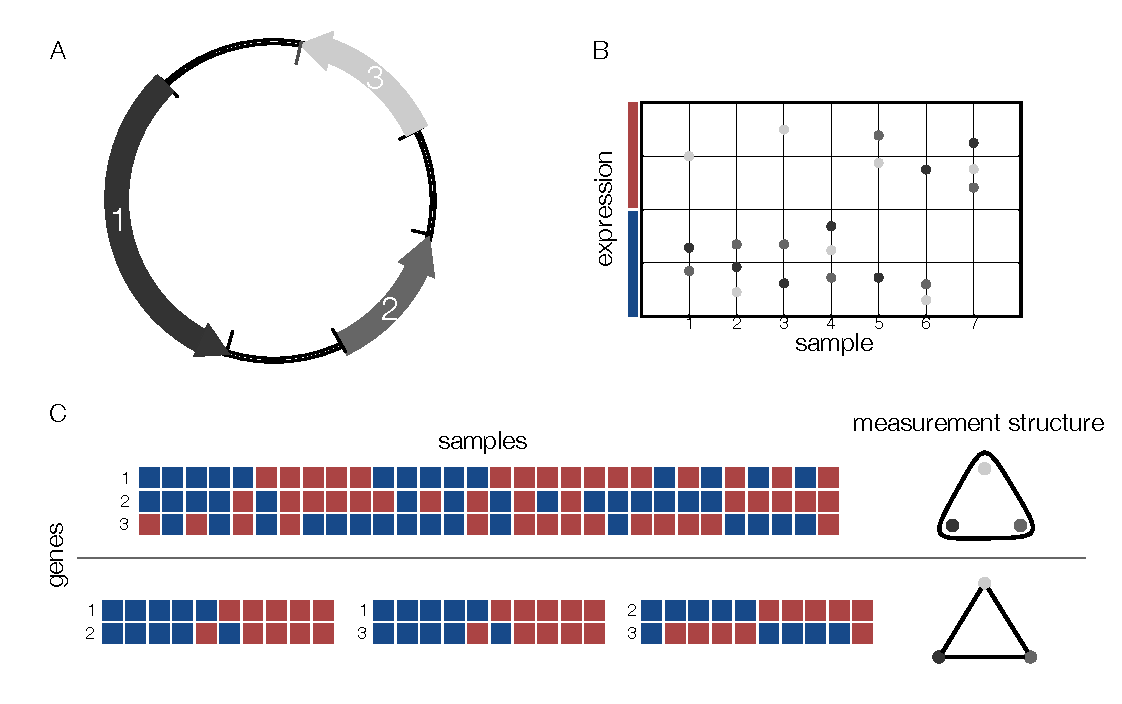
\includegraphics[width=0.9\columnwidth]{fig/figure_expression_concept.pdf}
\caption{{\bf Coarse-graining of gene expression data.} (A) Minimal representation of a small GRN consisting of three genes encoded in a plasmid. (B) Example binary coarse-graining of gene expression data. For each sample a measurement is taken for all three genes. The expression levels are binned into one of two classes represented by the red and blue bars representing relatively high and low expression respectively. (C) Heat map representation of coarse-grained gene expression data under the assumption of two different GRNAs. The samples on top and the associated measurement structure correspond to the case where constraints are placed on all three genes by a single element of the network context (\ref{fig:stochdynscheme} top row). The bottom represents the case where all three pairs of genes are each independently constrained by elements of the network context (\ref{fig:stochdynscheme} bottom row).}
\label{fig:expression_concept}
\end{figure}

\begin{figure}[!ht]
\centering
\noindent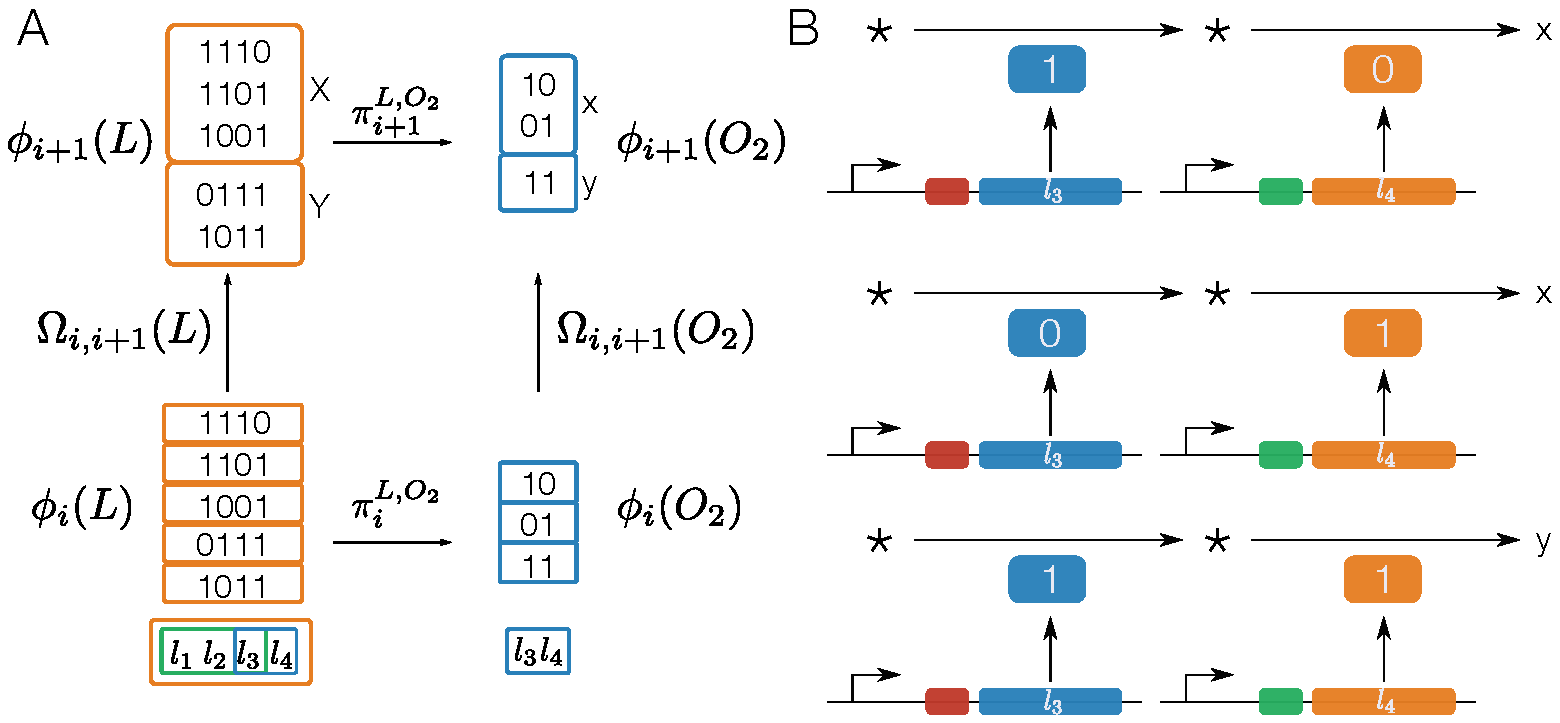
\includegraphics[width=0.9\columnwidth]{fig/phenotypehierarchy.pdf}
\caption{{\bf Example coarse-graining of phenotypes.} (A) Consider the example where $L = \{l_1,l_2,l_3,l_4\}$, $\mathcal{G} = \{ O_1, O_2 \}$, $O_1 = \{l_1, l_2, l_3\}$ and $O_2 = \{ l_3, l_4 \}$. The top left panel shows two higher-level phenotypes $X$ and $Y$. The bottom left corner shows the five different expression states of four genes in $L$ from which these phenotypes are coarse-grained. The right side shows the respective projections onto genes $\{l_3,l_4\}$. The projection maps $\pi_i^{L,O_2}$ and $\pi_{i+1}^{L,O_2}$ are defined in \refsupp{} \ref{secsupp:coarsegrainingphenotypes}. (B) The different combinations of expression states of genes $\{l_3,l_4\}$ result in two different phenotypes. If both genes are expressed metabolite $y$ is produced whereas if only one of the two genes is expressed metabolite $x$ is produced. The red and green boxes represent arbitrary promoters.}
\label{fig:phenotypehierarchy}
\end{figure}

\begin{figure}[!ht]
\centering
\noindent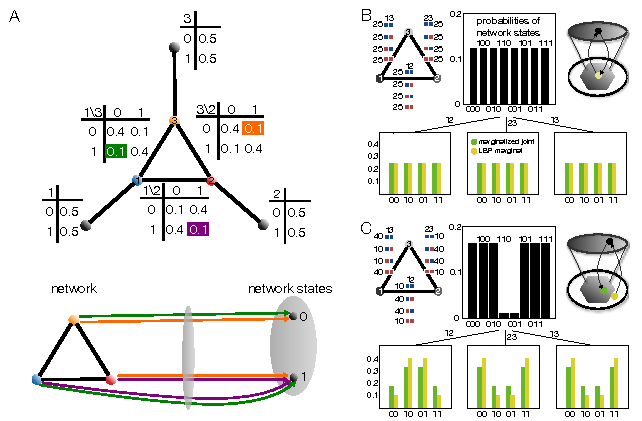
\includegraphics[width=0.9\columnwidth]{fig/inconsistentthreecycle.pdf}
\caption{{\bf Model of inconsistent gene expression data.} (A) An example structured according to \ref{fig:expression_concept}C bottom. The graph contains three nodes each representing one of the genes depicted in \ref{fig:expression_concept}A. The gray node coming from each node is placed next to the node marginal distribution depicted in the associated table. The edge marginal distributions are placed along the edges. The highlighted table entries (top) represent the constraint probabilities on the \gnpm{} represented by the equivalently colored arrows (bottom). The phenotype values derive from the coarse-graining process over gene expression data depicted in \ref{fig:expression_concept}B. (B) Given the model in panel A, the top-left panel represents three hundred samples comprising a data set consistent with a uniform distribution over all \gnpm{}. The top-middle panel represents the joint probability distribution determined via maximum-likelihood estimation with respect to the sufficient statistics (in this case, counts of pairwise observations of genes in states where blue corresponds to 0 and red corresponds to 1) given in the top-left panel. The green bars in the bottom three panels represent the marginalization of this joint distribution according to the structure of the graph. The yellow bars in the bottom three panels represent the ostensible marginal distributions determined via the sum-product algorithm (loopy belief propagation) \cite{Barber2012}. The top-right panel is a schematic where the top gray ellipse represents the space of joint probability distributions on three genes each with two expression states (i.e. $\Delta_7$: the eight-dimensional probability simplex) and the bottom ellipse represents the union of three copies of the four-dimensional probability simplex (i.e. $\Delta_3^{\oplus 3}$), one for each edge in the graph.  For this data, maximum likelihood estimation and loopy belief propagation yield equivalent points in $\Delta_3^{\oplus 3}$. (C) Same as B, but with data consistent with \ref{fig:expression_concept}C bottom, which in the limit of a large amount of data would converge to the ostensible node and edge marginal distributions in panel A of this figure. For this data, maximum likelihood estimation and loopy belief propagation yield different points in $\Delta_3^{\oplus 3}$.}
\label{fig:inconsistentthreecycle}
\end{figure}

\begin{figure}[!ht]
\centering
\noindent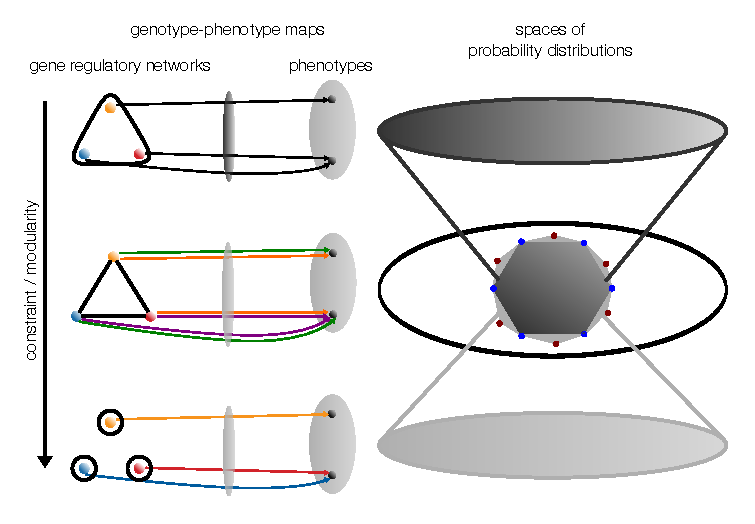
\includegraphics[width=0.9\columnwidth]{fig/conediagram.pdf}
\caption{{\bf Relationship between gene regulatory network models and spaces of probability distributions.} (A) The collection of all possible GRNAs over three genes forms a lattice represented here by its Hasse diagram. An analogous lattice of GRNAs exists for any number of genes. The Hasse diagram shows the manner in which GRNAs are hierarchically related and are thus able to be embedded within one another. (B) Explicit examples of \gnpm{} over three GRNAs from panel A highlighted in green are represented as arrows mapping the genes represented as nodes of the graph underlying the GRNA into the collection of phenotype values determined by the coarse-graining chosen in \ref{fig:expression_concept}B. There is a different collection of possible \gnpm{} depending upon the structure of the GRNA. (C) Each collection of \gnpm{} one representative for each GRNA depicted in panel B is associated to a space of probability distributions defined over it. Moreover, the spaces of probability distributions associated to each graph are related via marginalization maps. The top represents a joint probability distribution which can be marginalized to the middle space which in turn can be marginalized to the bottom space. The light gray polytope in the middle, $\mathbb{L}(\mathcal{G})$, represents the space of distributions consistent with the marginalization map from the middle to the bottom. The dark gray polytope, $\mathbb{M}(\mathcal{G})$, represents the space of probability distributions consistent with marginalization from the top to the middle.}
\label{fig:conediagram}
\end{figure}

% \begin{figure}[!ht]
% \centering
% \noindent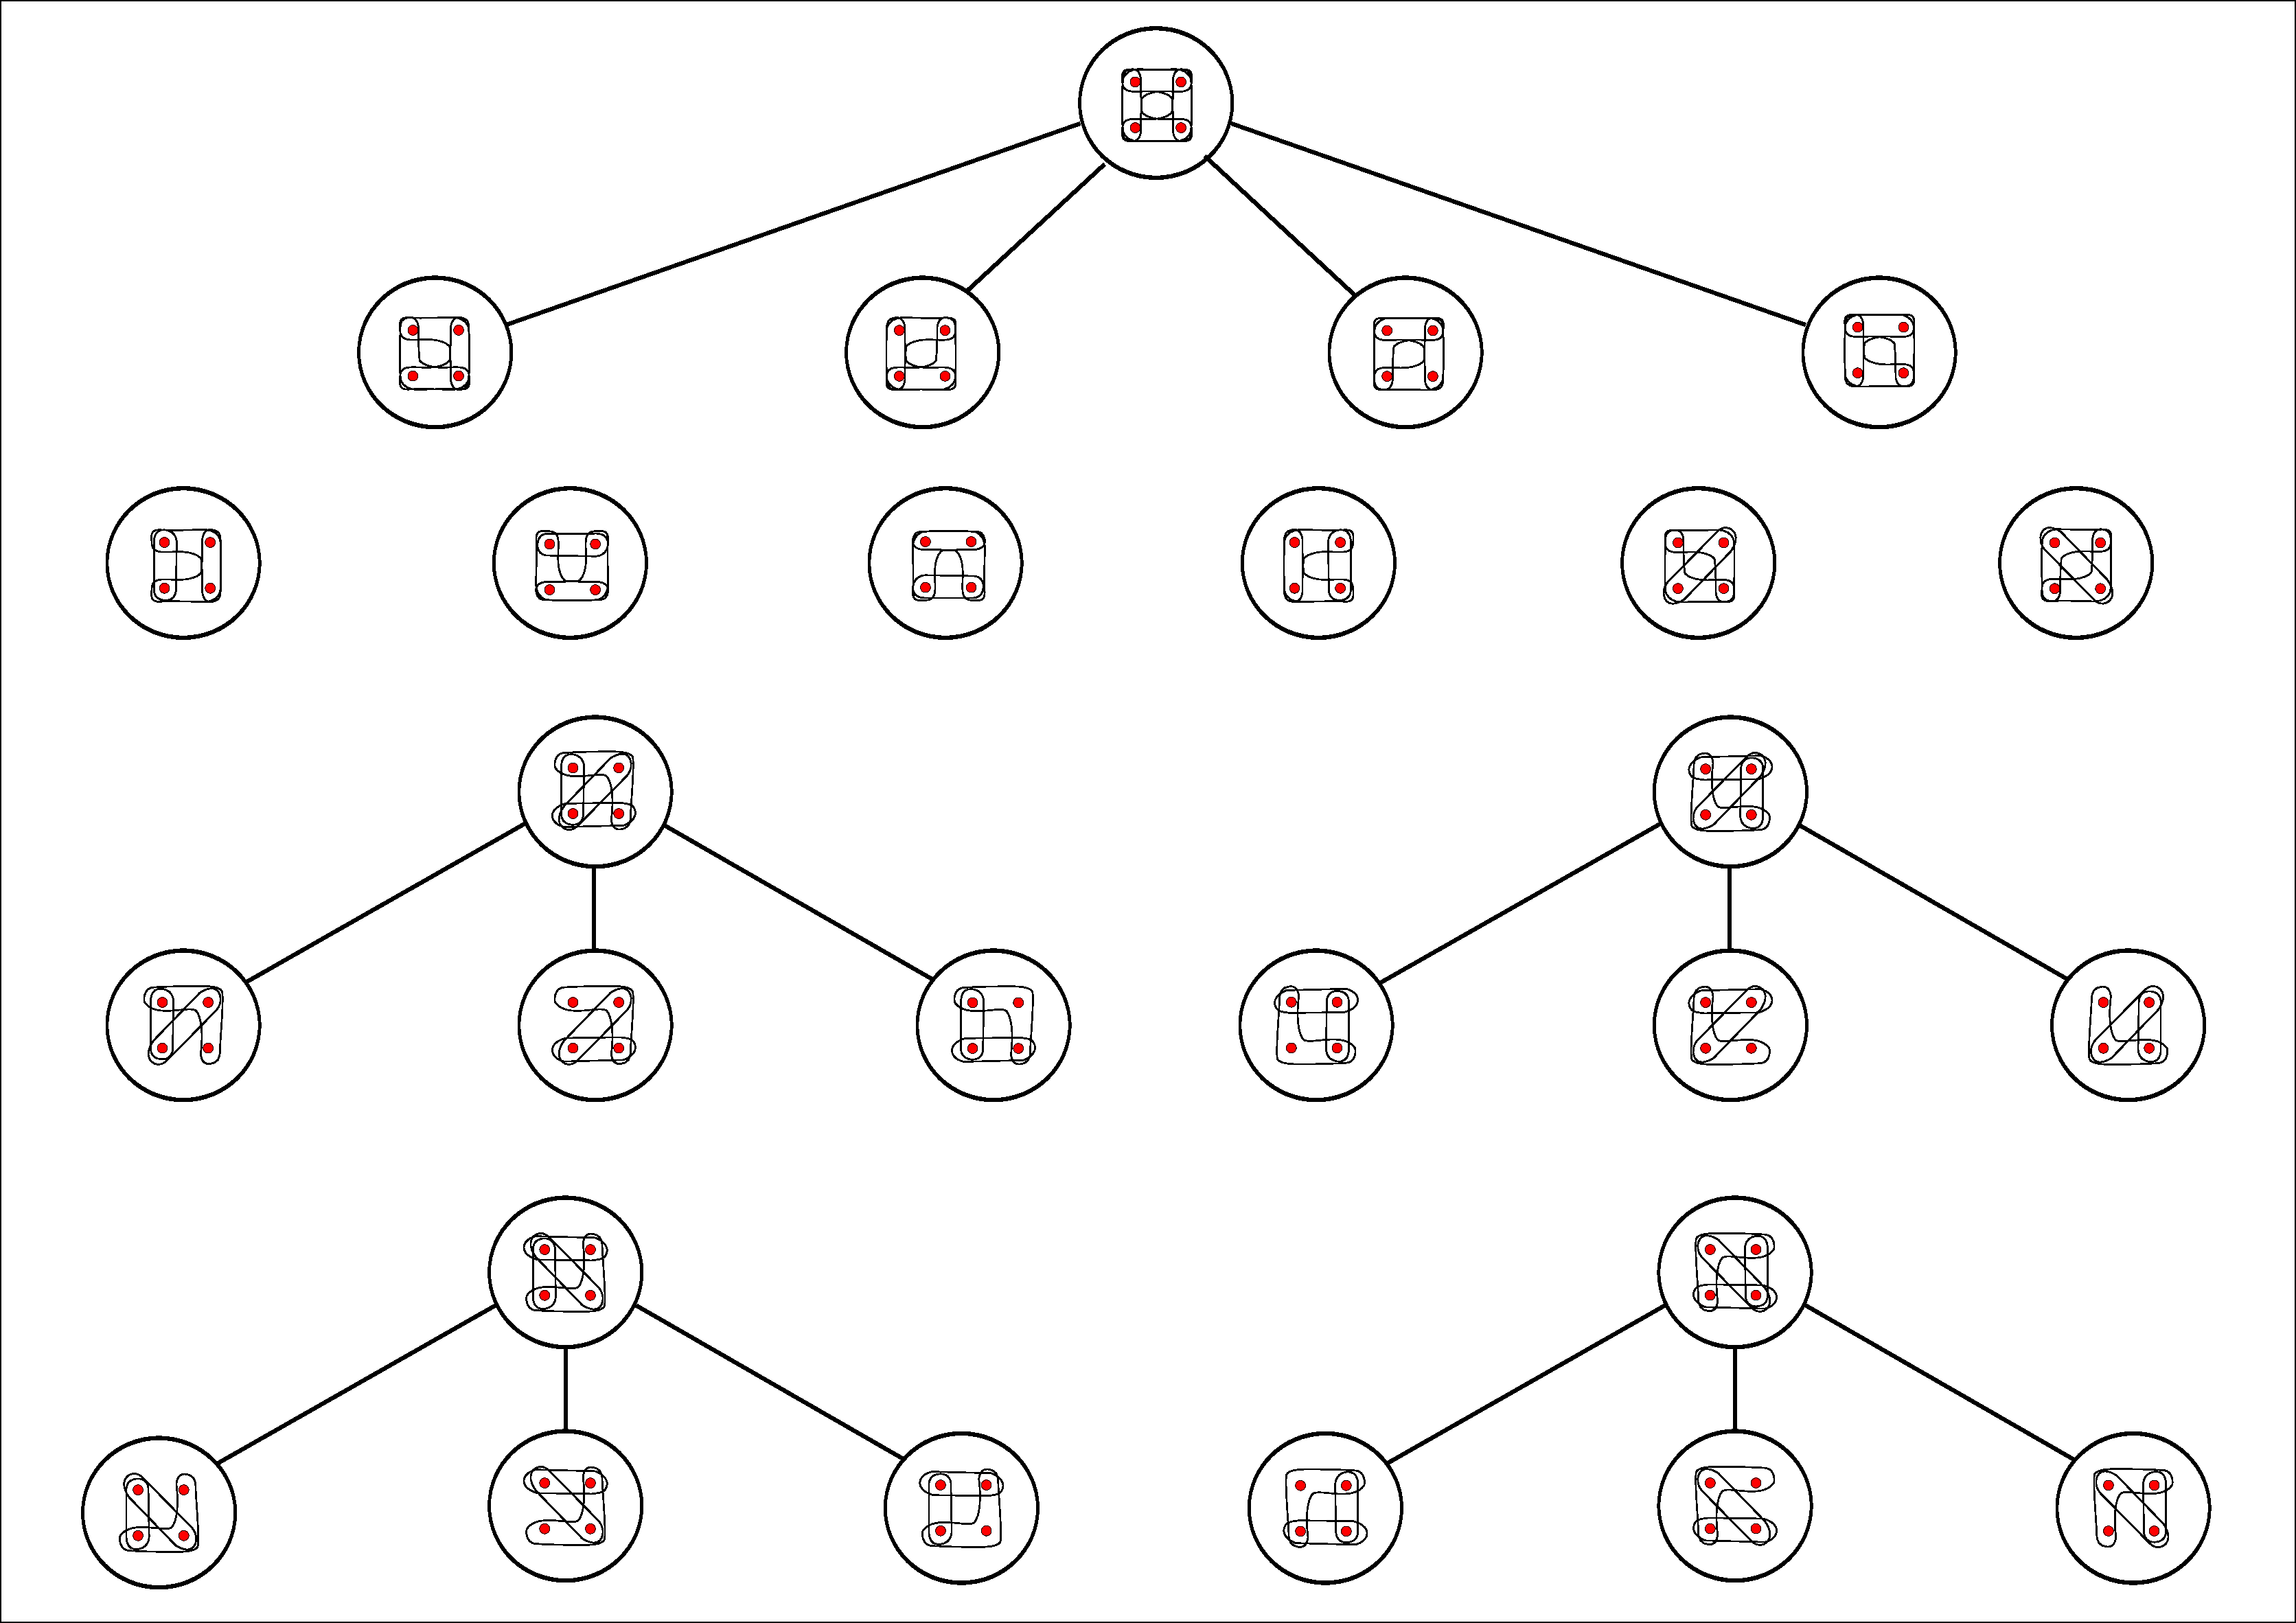
\includegraphics[width=1.0\columnwidth]{fig/non2uniformcyclichypergraphhasse.pdf}
% \caption{{\bf Hierarchical relationships among all possible classes of hypergraphs that are not graphs (i.e. not 2-uniform) but have cycles.} (A) There is a Hasse diagram for the lattice of GRNAs analogous to that of \ref{fig:conediagram}A but defined on four rather than only three genes. Within this lattice some of the graphs have cycles and some do not. (B) The highest levels of the Hasse diagram associated to the lattice of GRNAs on four genes containing hypergraphs having cycles. (C) and (D) contain lower levels of GRNAs containing cycles. Each of the four panels in (D) are on the same level. In total, each level represents an isomorphism class of hypergraphs. Therefore, there are five isomorphism classes of non-2-uniform hypergraphs representing GRNAs on four genes that contain cycles leading to the relationship between spaces of probability distsributions on associated genotype-phentoype maps analogous to that of \ref{fig:conediagram}C.}
% \label{fig:non2uniformcyclichypergraphhasse}
% \end{figure}

\begin{figure}[!ht]
\centering
\noindent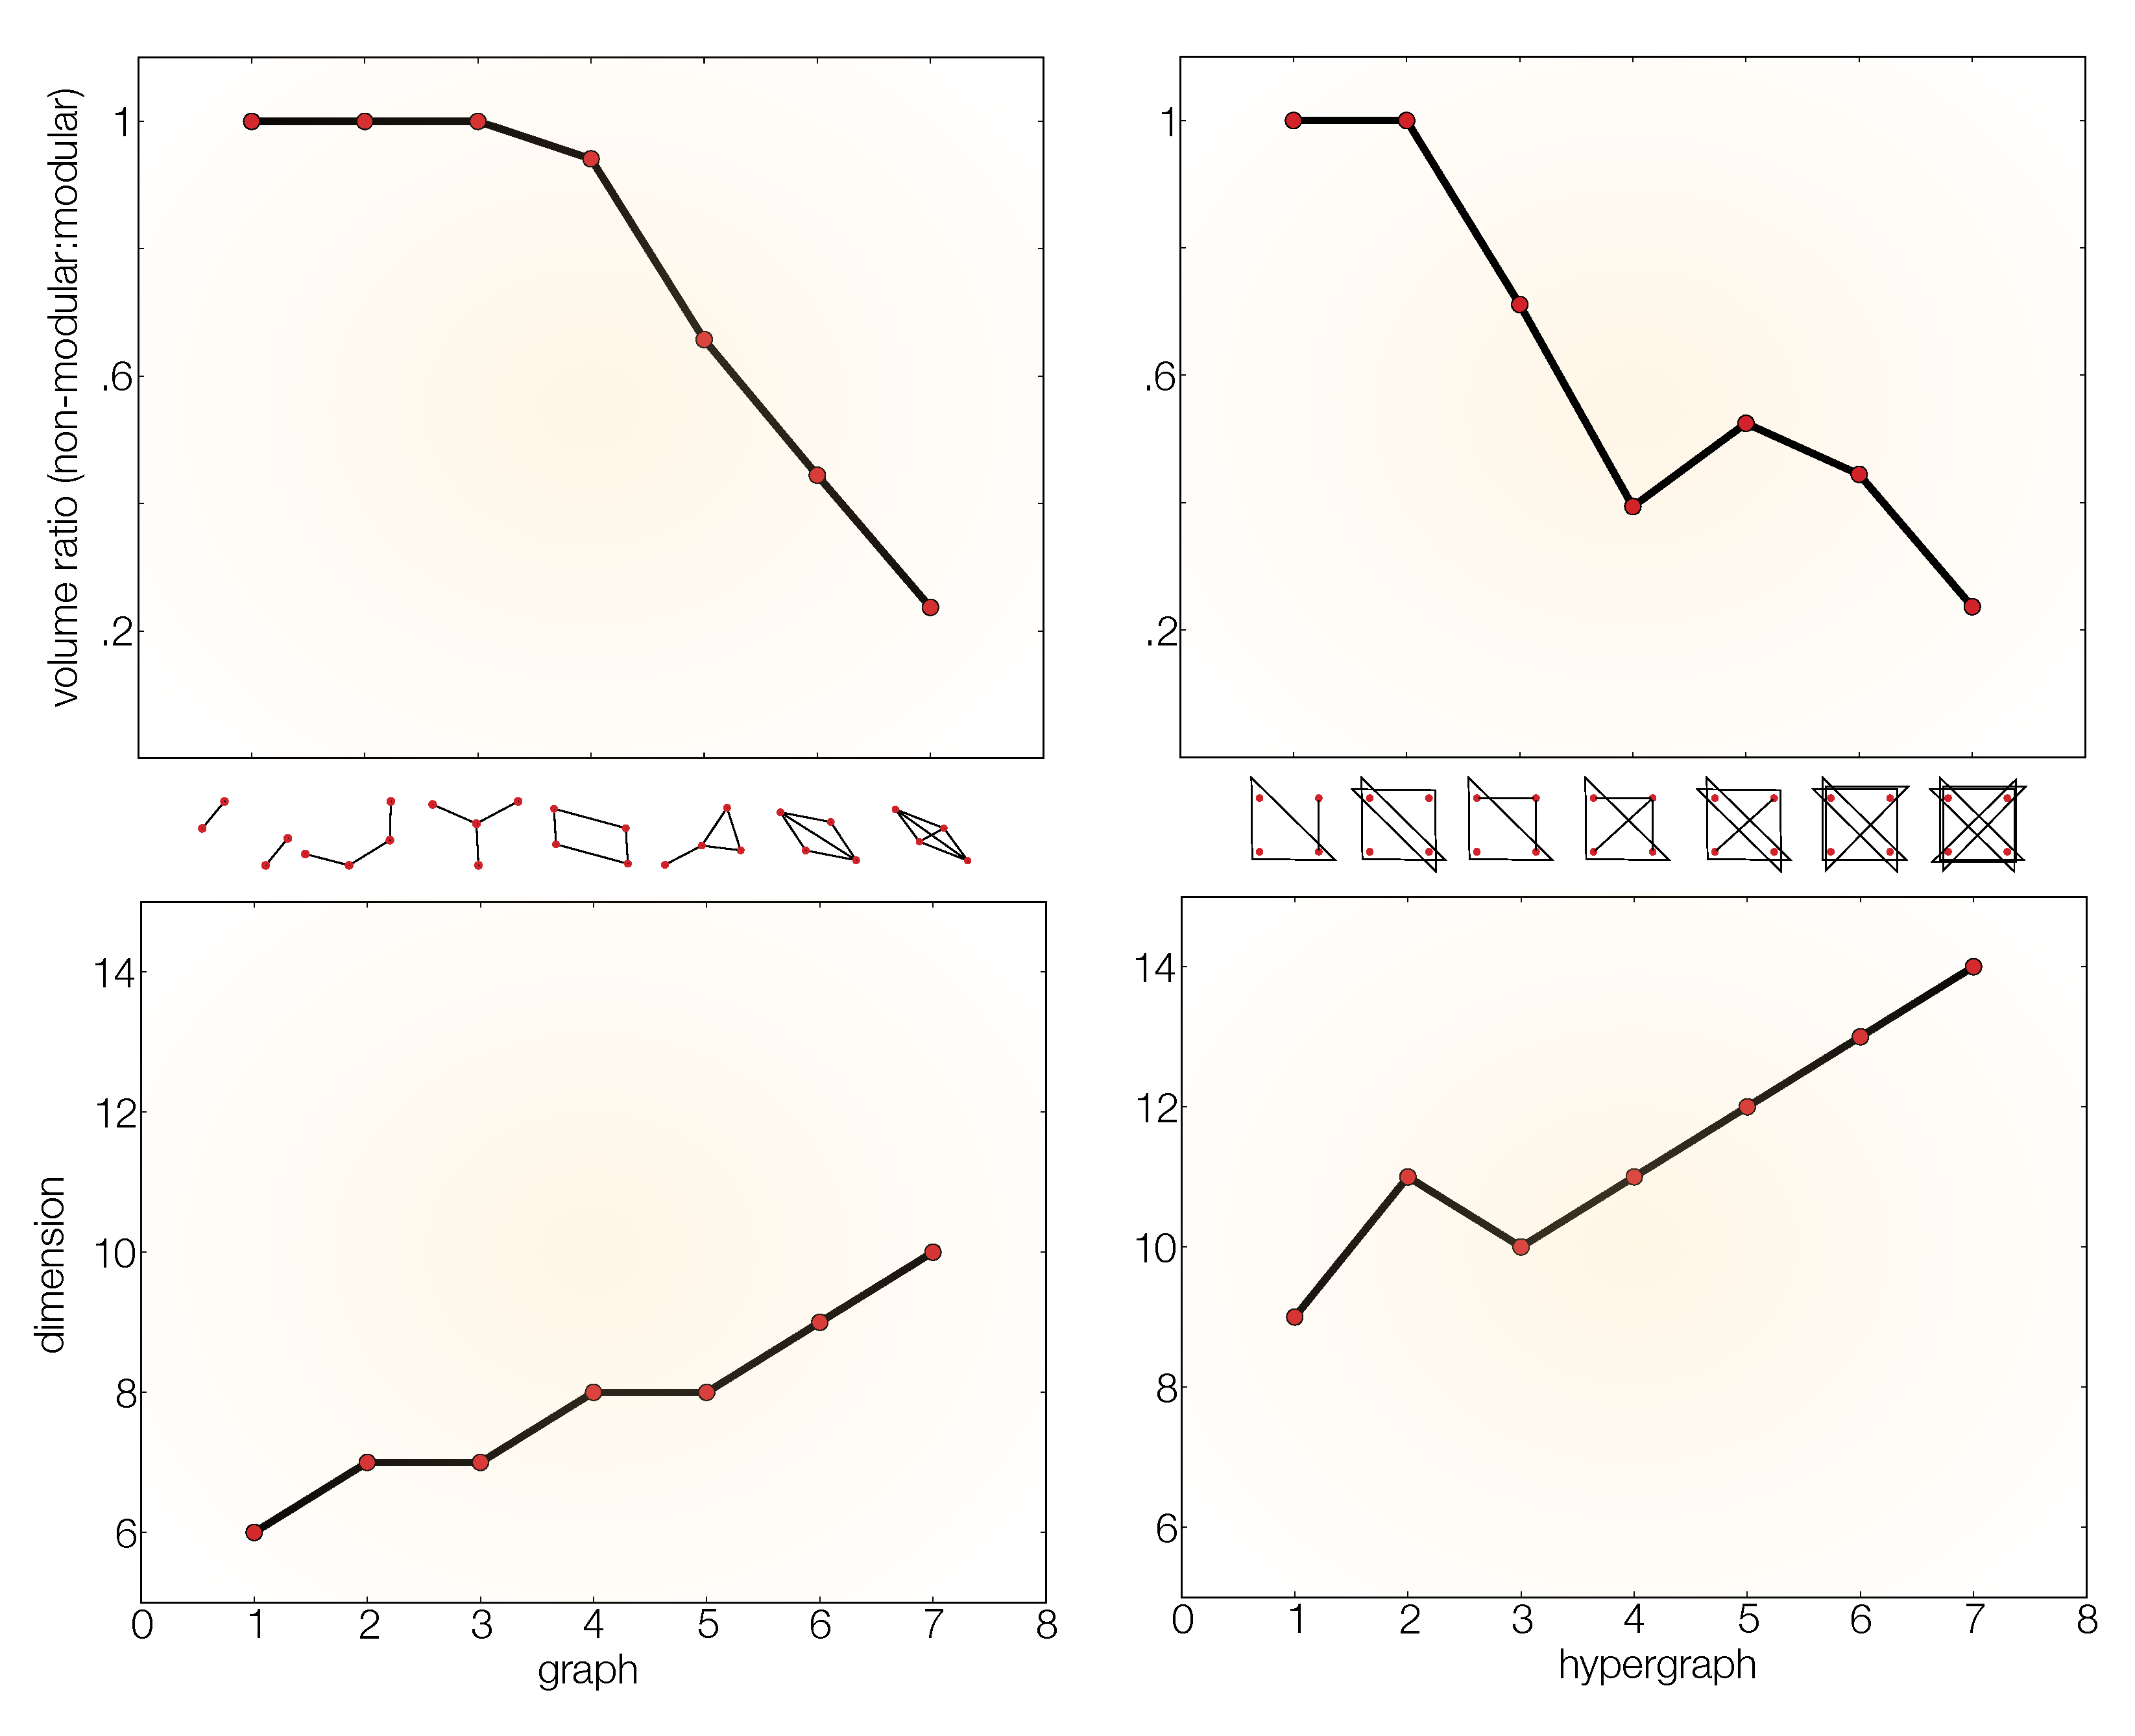
\includegraphics[width=0.9\columnwidth]{fig/figure_graphs_dims_nolines.pdf}
\caption{{\bf Non-modular to modular probability space volume ratio.} (A) and (B) show the ratio $\frac{\text{Vol}(\mathbb{M}(\mathcal{G}))}{\text{Vol}(\mathbb{L}(\mathcal{G}))}$ associated to 2-regular and non-2-regular GRNAs respectively. The (hyper)graph associated to each value of the volume ratio is displayed along the x-axis of each panel. (C) and (D) show the natural dimension of the space of probability distributions associated to $\mathbb{M}(\mathcal{G})$ and $\mathbb{L}(\mathcal{G})$ for each hypergraph.}
\label{fig:ncycvolrat}
\end{figure}

\begin{figure}[!ht]
\centering
\noindent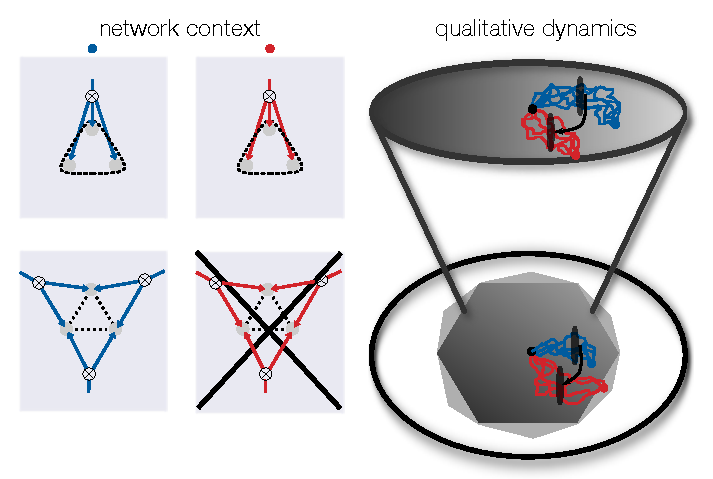
\includegraphics[width=0.9\columnwidth]{fig/stochdynscheme.pdf}
\caption{{\bf Schematic representation of the constraints imposed on stochastic gene expression and evolutionary dynamics by network architecture.} Schematic representation of a potential network context (left) for each of the hypothetical stationary probability distributions associated to the fitness peak established by the blue and red points within the spaces of probability distributions represented on the right. Algebraically, the top one corresponds to $\dist (\expr (L))$ and the bottom to $\dist (\expr (\mathcal{G}))$. Either of the two GRNAs represented on the left are capable of achieving the stationary distribution over \gnpm{} specified by the blue stationary distribution associated to a hypothetical fitness peak. On the other hand, only the GRNA from the top (and not the bottom) is capable of achieving the red stationary distribution representing an alternative potential fitness peak.}
\label{fig:stochdynscheme}
\end{figure}
